\documentclass[11pt,          % font size: 11pt or 12pt
               phd,           % degree:    ms or phd
               onehalfspacing % spacing: onehalfspacing or doublespacing
               ]{ncsuthesis}

%%----------------------------------------------------------------------------%%
%%------------------------------ Import Packages -----------------------------%%
%%----------------------------------------------------------------------------%%

\usepackage{booktabs}  % professionally typeset tables
\usepackage{amsmath}
\usepackage{textcomp}  % better copyright sign, among other things
\usepackage{xcolor}
\usepackage{lipsum}    % filler text
\usepackage{subfig}    % composite figures


%%----------------------------------------------------------------------------%%
%%---------------------------- Formatting Options ----------------------------%%
%%----------------------------------------------------------------------------%%
%%

%% -------------------------------------------------------------------------- %%
%% Disposition format -- any titles, headings, section titles
%%  These formatting commands affect all headings, titles, headings,
%%  so sizing commands should not be used here.
%%  Formatting options to consider are
%%     +  \sffamily - sans serif fonts.  Dispositions are often typeset in
%%                    sans serif, so this is a good option. 
%%     +  \rmfamily - serif fonts
%%     +  \bfseries - bold face
%\dispositionformat{\sffamily\bfseries}   % bold and sans serif
\dispositionformat{\bfseries}            % bold and serif

%% -------------------------------------------------------------------------- %%
%% Formatting for centered headings - Abstract, Dedication, etc. headings
%%  This is where one might put a sizing command.
%%  \MakeUppercase can be used to typeset all headings in uppercase.
\headingformat{\large\MakeUppercase}   % All letters uppercase
%\headingformat{\large}                % Not all uppercase
%\headingformat{\Large\scshape}        % Small Caps, used with serif fonts.

%% Typographers recommend using a normal inter-word space after
%% sentences. TeX's default is to add an wider space, but \frenchspacing
%% gives a normal spacing. Comment out the following line if you prefer
%% wider spaces between sentences.
\frenchspacing


%% -------------------------------------------------------------------------- %%
%%  Optional packages
%%    A number of compatible packages to improve the look and feel of
%%    your document are available in the file optional.tex 
%%    (For example, hyperlinks, fancy chapter headings, and fonts)
%% To use these options, uncomment the next line and see optional.tex
%%%  Optional Packages to consider.   These packages are compatible with
%%    ncsuthesis.  

%% -------------------------------------------------------------------------- %%
%% Fancy chapter headings
%%  available options: Sonny, Lenny, Glenn, Conny, Rejne, Bjarne
%\usepackage[Sonny]{fncychap}
\usepackage[Rejne]{fncychap}

%%----------------------------------------------------------------------------%%
%% Hyperref package creates PDF metadata and hyperlinks in Table of Contents
%%  and citations.  Based on feedback from the NCSU thesis editor, 
%%  the links are not visually distinct from normal text (i.e. no change
%%  in color or extra boxes).
\usepackage[
  pdfauthor={Carlos Pompeyo Ortiz},
  pdftitle={Rigidity of Microsphere Heaps},
  pdfcreator={pdftex},
  pdfsubject={NC State ETD Thesis},
  pdfkeywords={microfluidics, hard sphere, jamming, suspension, rigidity, friction, microscopy},
  colorlinks=true,
  linkcolor=black,
  citecolor=black,
  filecolor=black,
  urlcolor=black,
]{hyperref}


%% -------------------------------------------------------------------------- %%
%% Microtype - If you use pdfTeX to compile your thesis, you can use
%%              the microtype package to access advanced typographic
%%              features.  By default, using the microtype package enables
%%              character protrusion (placing glyphs a hair past the right 
%%              margin to make a visually straighter edge)
%%              and font expansion (adjusting font width slightly to get 
%%              more favorable justification).
%%              Using microtype should decrease the number of lines
%%              ending in hyphens.
\usepackage{microtype}


%%----------------------------------------------------------------------------%%
%% Fonts 

%% ETD guidelines don't specify the font.  You can enable the fonts
%%  by uncommenting the appropriate lines.  Using the default Computer 
%%  Modern fonts is *not* required.  A few common choices are below.
%%  See http://www.tug.dk/FontCatalogue/ for more options.

%% Serif Fonts -------------------------------------------------
%%  The four serif fonts listed here (Utopia, Palatino, Kerkis,
%%  and Times) all have math support.


%% Utopia
\usepackage[T1]{fontenc}
\usepackage[adobe-utopia]{mathdesign}

%% Palatino
%\usepackage[T1]{fontenc}
%\usepackage[sc]{mathpazo}
%\linespread{1.05}

%% Kerkis
%\usepackage[T1]{fontenc}
%\usepackage{kmath,kerkis}

%% Times
%\usepackage[T1]{fontenc}
%\usepackage{mathptmx}


%% Sans serif fonts -------------------------

%\usepackage[scaled]{helvet}  % Helvetica
%\usepackage[scaled]{berasans} % Bera Sans



%%----------------------------------------------------------------------------%%
%%---------------------------- Content Options -------------------------------%%
%%----------------------------------------------------------------------------%%
%% Size of committee: 3, 4, 5, or 6 -- this number includes the chair
\committeesize{4}

%% Members of committee
%%  Each of the following member commands takes an optional argument
%%   to specify their role on the committee.
%%  For co-chairs, use the commands:
%%      \cochairI{Doug Dodd}
%%      \cochairII{Chris Cox}
%%
\chair{Doug Dodd}
\memberI{Alex Anderson}
\memberII{Bobby Brown}
\memberIII{Chris Cox}   % unnecessary if committeesize=3
\memberIV{Fred Ford}    % unnecessary if committeesize=3 or 4
\memberV{Edna Everitt}  % unnecessary if committeesize=3, 4, or 5


%% Student writing thesis, \student{First Middle}{Last}
\student{John Mark}{Smith} % a full middle name
%\student{John M.}{Smith} % a middle initial

%% Degree program
\program{Nuclear Engineering}

%% Thesis Title
%%  Keep in mind, according to ETD guidelines:
%%    +  Capitalize first letter of important words.
%%    +  Use inverted pyramid shape if title spans more than one line.
%%
%%  Note: To break the title onto multiple lines, use \break instead of \\.
\thesistitle{A North Carolina State University Sample \LaTeX{} Thesis \break 
with a Title So Long it Needs a Line Break}

%% Degree year.  Necessary if your degree year doesn't equal the current year.
%\degreeyear{1995}


%%----------------------------------------------------------------------------%%
%%---------------------------- Personal Macros -------------------------------%%
%%----------------------------------------------------------------------------%%

%% A central location to add your favorite macros.

%% A few examples to get you started.
\newcommand{\uv}[1]{\ensuremath{\mathbf{\hat{#1}}}}
\newcommand{\bo}{\ensuremath{\boldsymbol{\Omega}}}
\newcommand{\eref}[1]{Eq.~\ref{#1}}
\newcommand{\fref}[1]{Figure~\ref{#1}}
\newcommand{\tref}[1]{Table~\ref{#1}}

%%---------------------------------------------------------------------------%%
\begin{document}

%%---------------------------------------------------------------------------%%
\frontmatter

%% ------------------------------ Abstract ---------------------------------- %%
\begin{abstract}

\lipsum[1-6]


\end{abstract}


%% ---------------------------- Copyright page ------------------------------ %%
%% Comment the next line if you don't want the copyright page included.
\makecopyrightpage

%% -------------------------------- Title page ------------------------------ %%
\maketitlepage

%% -------------------------------- Dedication ------------------------------ %%
\begin{dedication}
 \centering To my parents.
\end{dedication}

%% -------------------------------- Biography ------------------------------- %%
\begin{biography}
The author was born in a small town \ldots
\end{biography}

%% ----------------------------- Acknowledgements --------------------------- %%
\begin{acknowledgements}
I would like to thank my advisor for his help.
\end{acknowledgements}


\thesistableofcontents

\thesislistoftables

\thesislistoffigures


%%---------------------------------------------------------------------------%%
\mainmatter

\chapter{INTRODUCTION}
\label{chap-one}
In this data explosion era, there are myriad programs that are executed repeatedly on large sets of data, consuming high amounts of energy and resources. Critical process reused on different data sets will no doubt help reduce the time and computations. In this work we will introduce a new probabilistic model of measuring data similarities. Based on these data similarities we will show how critical computations may be reused across data sets, saving energy and improving performance.

Our work will introduce a general architecture for comparing two or more data sets and get a probabilistic measure of similarity. We reason that if two data sets are similar, computation reuse from previous iteration of an algorithm for the similar data set will provide a good speed up in the execution of the algorithm for the current data set.
We first define the architecture to compute the above-mentioned metric of similarity and then proceed to validate our above-mentioned stipulation for the K-Means and the SGD based SVM algorithms.

In these explorations, we found challenges in 4 aspects: \textbf{data features, similarity definition, scalability,} and \textbf{reuse}. Data features, is the description of data sets. Similarity definition (distance between two data sets) is the metric we use to describe similarity between data sets. Data feature and distance definition are used together for reuse instance selection from a program specific database. The selection of history record is the most essential part of computation reuse.

Since the method used to calculate distances between two data sets, should also be defined based on data features, the problem becomes even more complex. Scalability issues are related with number of instances in database, size of the target data set, and dimension of data-set. Goal of computation reuse is to save computation time and energy. In order to select a suitable history record, some extra computation is inevitably introduced. The dilemma is the trade-off between the amount of computation reuse and the introduced overhead. 

Reuse, thus is the process to decide what history information the program should reuse and how to reuse the pre-computed information.
In this study we introduce the concept of Historical Computation reuse. This is an Intuitive Idea whose exploration for the family of algorithms mentioned above is spotted at best.

\textbf{\textit{Computation Reuse}} is the process of deciding what history information the program should reuse and how to best reuse the pre-computed information.
While the idea is simple and intuitive in nature, it promises big gains if correctly implemented with a wide variety of uses.
In this study we give an empirical study, showing that effectively computation reuse could enhance program performance.
Although, the idea of computation reuse is simple, there are many difficulties need to be solved to achieve efficient and effective reuse. 
In our explorations, we found out challenges in 4 aspects: data feature abstraction, similarity definition, scalability, and reuse. 
\textit{Data Features}, is the description of data sets. The major challenged we faced in \textit{Data Feature Abstraction} was to reduce dimensionality (for the sake of optimization), while preserving the integrity of data.
\textit{Similarity definition} (distance between two data-sets) is the way we would like to describe similarity between two data set. The challenge was to come up with a meaningful metric to give an accurate prediction of suitability for reuse. 
We used \textit{Data feature abstraction} and \textit{Similarity definition} together for reuse instance selection from a program specific database. The selection of history data set is the most essential part of computation reuse because different data sets will lead to dramatically different computation times. Because the most important properties of the input data may vary on different programs, it is difficult to decide a universal data feature and data distance definition. Since the method used to calculate distances between two data sets descriptions also should be defined based on the data features, the problem becomes even more complicated. 
\textit{Scalability} issues are related with number of data set instances in database, size of the target data set, and its dimensionality. Goal of computation reuse is to save computation time and energy. In order to select a suitable history record, some extra computation is inevitably introduced into the computation. The dilemma is the tradeoff between the amount of computation reuse and the introduced overhead. For example, increase the number of instances in database will increase the probability of finding a good history record. However, it will also increase the introduced selection overhead. The size of target data set and the dimensionality of would also produce similar issues.
\textit{Reuse} is the process of deciding what history information the program should reuse and how to reuse this pre-computed information. Challenges in this field are mainly caused by the differences among programs and algorithms. For a specific program or algorithm, it might be a trivial solution while for another selecting historical data may be a complex problem. Our approach of building a general framework to work as a plug and play device makes the process even more complicated. 
In this work, we investigate multiple solutions to address each of the challenges, and come up a framework, which we will apply to two of commonly used algorithms, namely: \textbf{\textit{K-Means(Lloyd’s Clustering algorithm)}} and the \textbf{\textit{Stochastic Gradient Decent based Support Vector Machine}} for our explorations and providing proof of effectiveness of History Reuse and to validate the efficiency and the effectiveness of our algorithm.
The paper is organized in the following sections: \textit{\ref{chap-two}} gives motivation, background and definitions of terms we use in this paper. \textit{\ref{chap-three}} will give formal definition to the challenges we faced and our approach for coming to a successful conclusion. \textit{\ref{chap-four}} will formalize the framework and give the formal algorithm for our architecture. We will also discuss the other approaches we used to come to our conclusions and give reasons for their failures. We present the evaluations for our algorithm in \textit{\ref{chap-five}}. Related and future work is discussed in \textit{\ref{chap-six}}, while \textit{\ref{chap-seven}} provides conclusion derived from our explorations.

\chapter{Tables, Figures and Matrices}
\label{chap-two}
In Chapter \ref{chap-one} we did some typesetting and equations; now let's 
look at tables, figures, and matrices.

\section{Tables}
Table \ref{tab:one} is about as simple as they come, to put a formula in a 
table just use the same methods as putting a formula in a paragraph.  
Table \ref{tab:two} is a similar table in landscape on a seperate page.  
%
\begin{table}
\caption{Table Example}
\label{tab:one}
\begin{center}
\begin{tabular}{lccl}
\toprule
Treatment & No Death & Death & Total\\
\midrule
Therapy A & 1295 & 72 & 1367\\
Therapy B 	& 2294 & 195 & 2489\\
\midrule
Total & 3589 & 267 & 3856\\
\bottomrule
\end{tabular}
\end{center}
\end{table}

\paragraph{Filler Text} \lipsum[1-2]

\begin{lscape}
\begin{table}
\caption{Landscape Table Example}
\label{tab:two}
\begin{center}
\begin{tabular}{lcccccccccl}
\toprule
Patient & A & B & C & D & E & F & G & H &I & Total \\
\midrule
John & 1 & 2 & 3 & 4 & 5 & 6 & 7 & 8 & 9 & 45 \\
Amy & 1 & 2 & 3 & 4 & 5 & 6 & 7 & 8 & 9 & 45 \\
Jim & 1 & 2 & 3 & 4 & 5 & 6 & 7 & 8 & 9 & 45 \\
Jason & 1 & 2 & 3 & 4 & 5 & 6 & 7 & 8 & 9 & 45 \\
Sandy & 1 & 2 & 3 & 4 & 5 & 6 & 7 & 8 & 9 & 45 \\
Icem & 1 & 2 & 3 & 4 & 5 & 6 & 7 & 8 & 9 & 45 \\
\midrule
Total & 6 & 12 & 18 & 24 & 30 & 36 & 42 & 48 & 54 & 270\\
\bottomrule
\end{tabular}
\end{center}
\end{table}
\end{lscape}


\section{Figures}

The easiest way to insert a picture is to have that picture in pdf format.  
\fref{fig:hist1} and \fref{fig:hist2} are two figures typeset normally.
ETD guidelines allow the use of landscape pages in the electronic 
submission.  To rotate a page, use the \texttt{lscape} environment.
Please note, if you are preparing a document for binding, consider
giving the \texttt{hardcopy} option in the \verb|\documentclass|
declaration.  This will place the page number at the normal location,
which is where it should be for printing and binding.
%
\begin{figure}[hbtp]
\centering
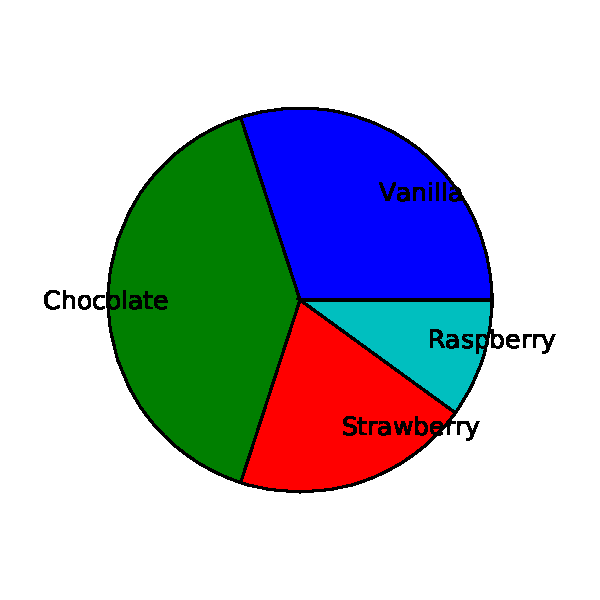
\includegraphics[width=0.6\textwidth]{Chapter-2/figs/pie}
\caption{Here is a sample figure}
\label{fig:hist1}
\end{figure}
%
\begin{figure}[hbtp]
\centering
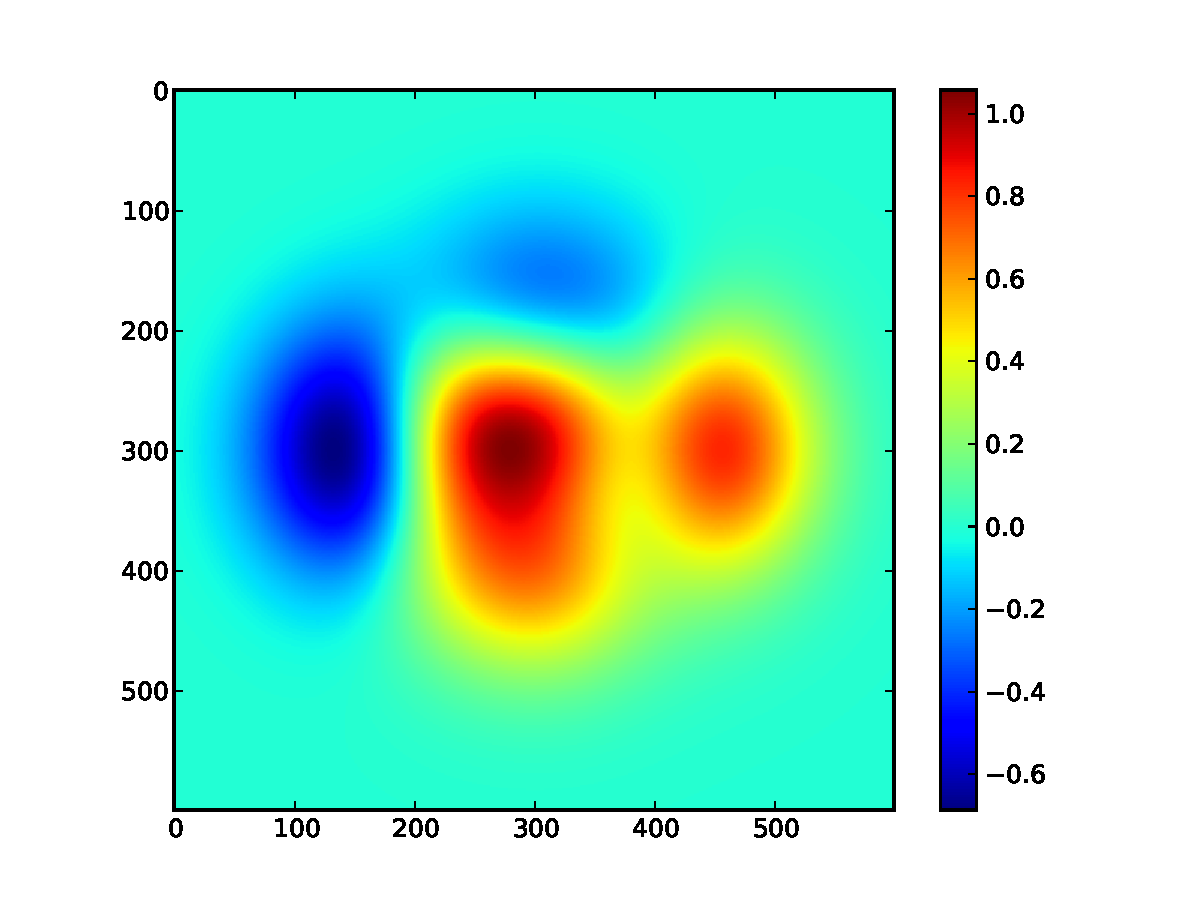
\includegraphics[width=0.6\textwidth]{Chapter-2/figs/color}
\caption{Here is a sample figure}
\label{fig:hist2}
\end{figure}
%
\begin{figure}[hbtp]
\centering
\subfloat[]{
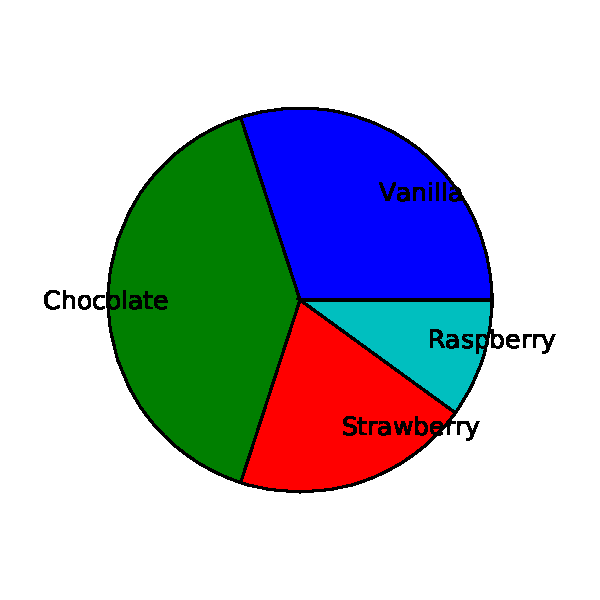
\includegraphics[width=0.4\textwidth]{Chapter-2/figs/pie}
}
\subfloat[]{
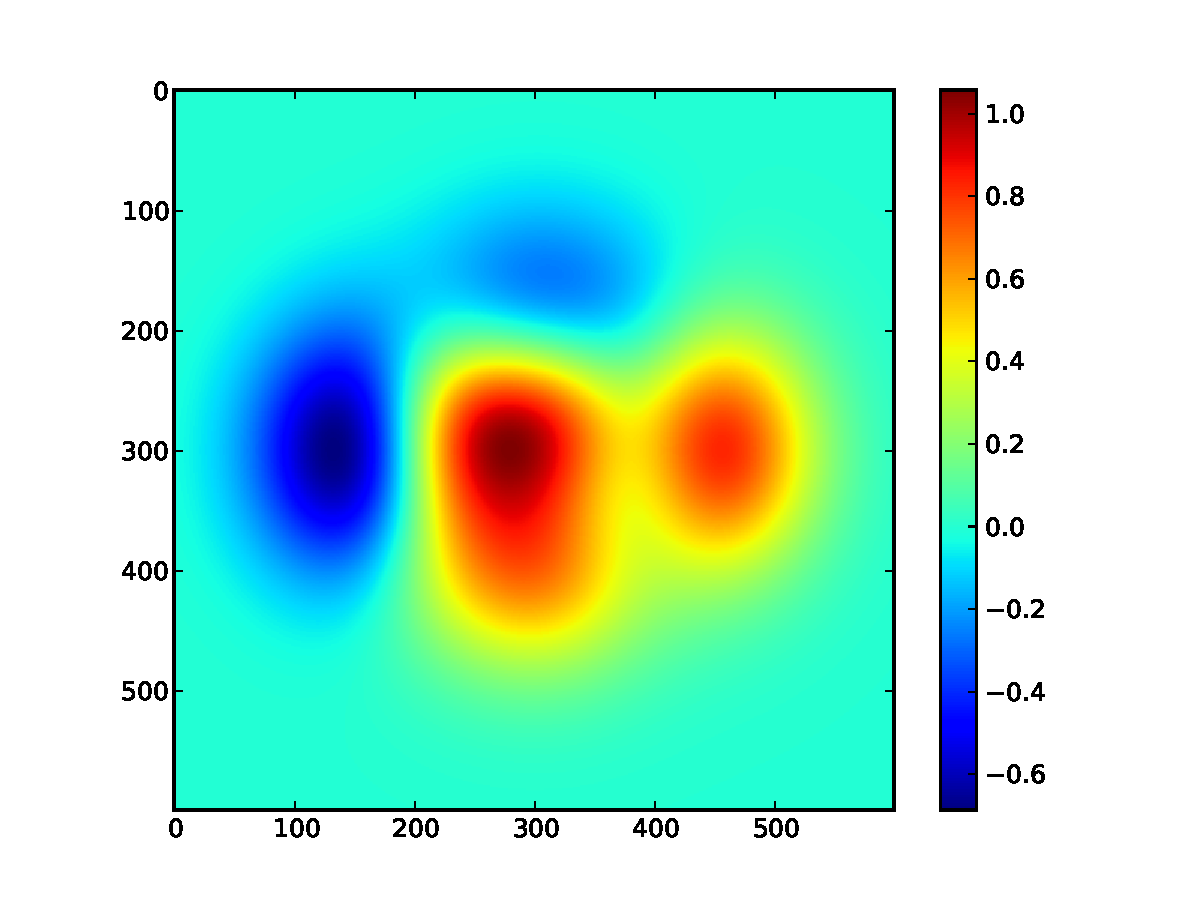
\includegraphics[width=0.4\textwidth]{Chapter-2/figs/color}
}
\caption{Here are two floating subfigures}
\label{fig:subfigures}
\end{figure}


\paragraph{Filler Text} \lipsum[12-15]

\begin{lscape}
\begin{figure}
\centering
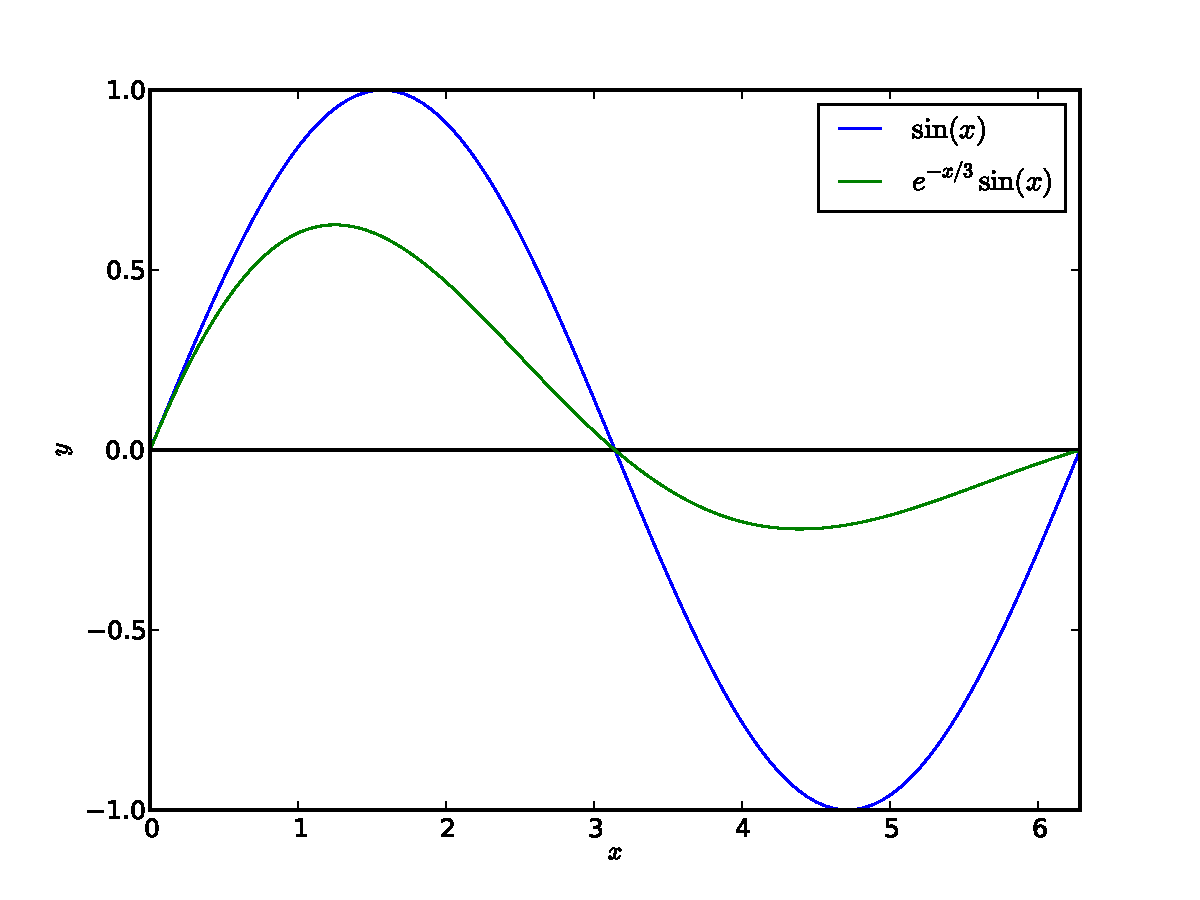
\includegraphics[width=\textwidth]{Chapter-2/figs/sine}
%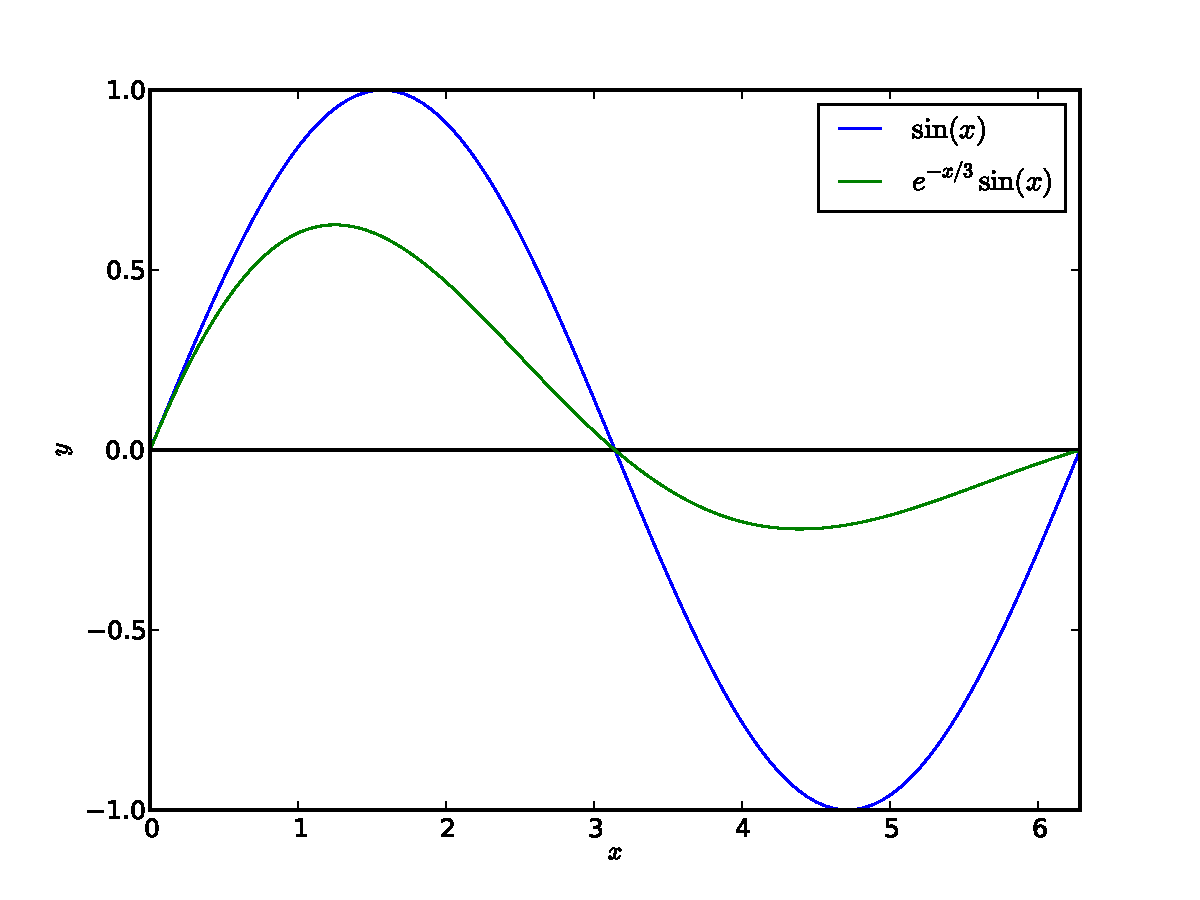
\includegraphics[height=\textwidth]{Chapter-2/figs/sine}
\caption{This figure has been turned sideways.  With large figures, 
         the author must ensure that there are at least two double spaces
         between the caption and the page number.}
\label{fig:hist}
\end{figure}
\end{lscape}

\section{Matrices}
Let's look at a simple example of a matrix:
\[ \left( \begin{array}{ccc}
a & b & c \\
d & e & f \\
g & h & i \end{array} \right)\] 
%
You may prefer to write it this way:
\[ \left[\begin{array} {cccccc}
1 & 0 & 0 & 0 & 0 & 0 \\
0 & 1 & 0 & 0 & 0 & 0 \\
0 & 0 & 1 & 0 & 0 & 0 \\
0 & 0 & 0 & 1 & 0 & 0 \\
0 & 0 & 0 & 0 & 1 & 0 \\
0 & 0 & 0 & 0 & 0 & 1 \\
\end{array} \right] \]

\chapter{Lorem Ipsum}

\section*{A First Section}

\paragraph{Filler Text} \lipsum[1-6]
%
\begin{figure}[t]
  \centering
  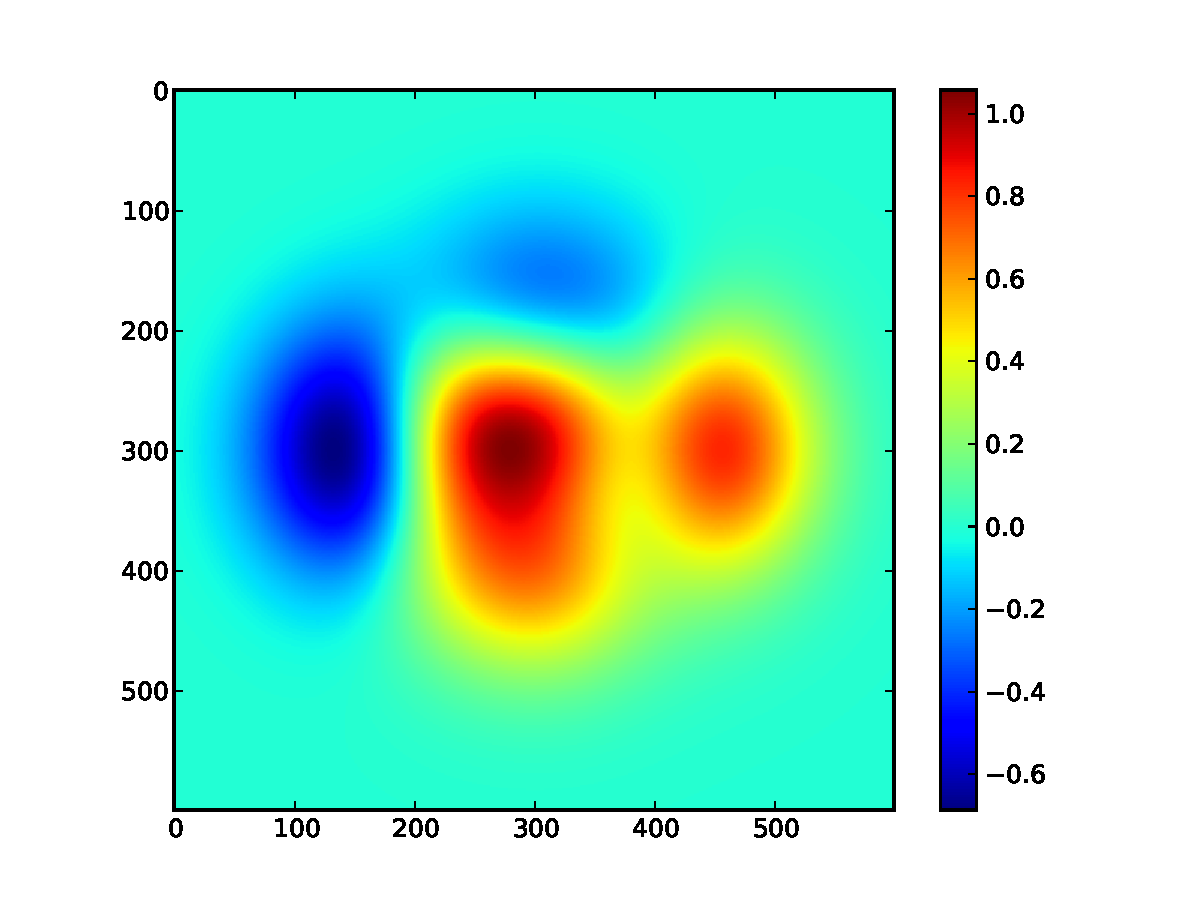
\includegraphics[width=0.6\textwidth]{Chapter-2/figs/color}
  \caption{A figure at the top of the page.}
  \label{fig:ch3.1}
\end{figure}
%
\lipsum[7-13]
%
\begin{figure}[!h]
  \centering
  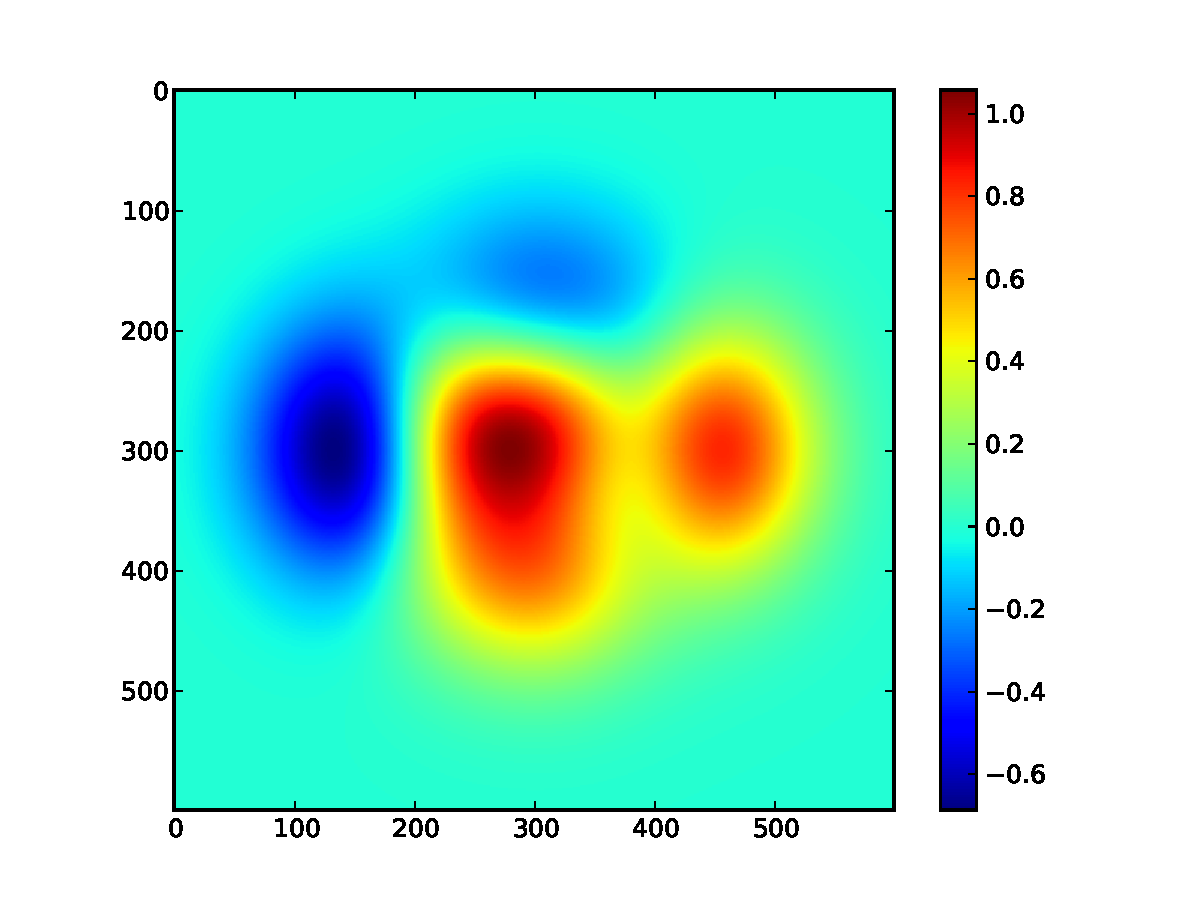
\includegraphics[width=0.6\textwidth]{Chapter-2/figs/color}
  \caption{A figure in the middle of text.}
  \label{fig:ch3.2}
\end{figure}
%
\begin{figure}[!b]
  \centering
  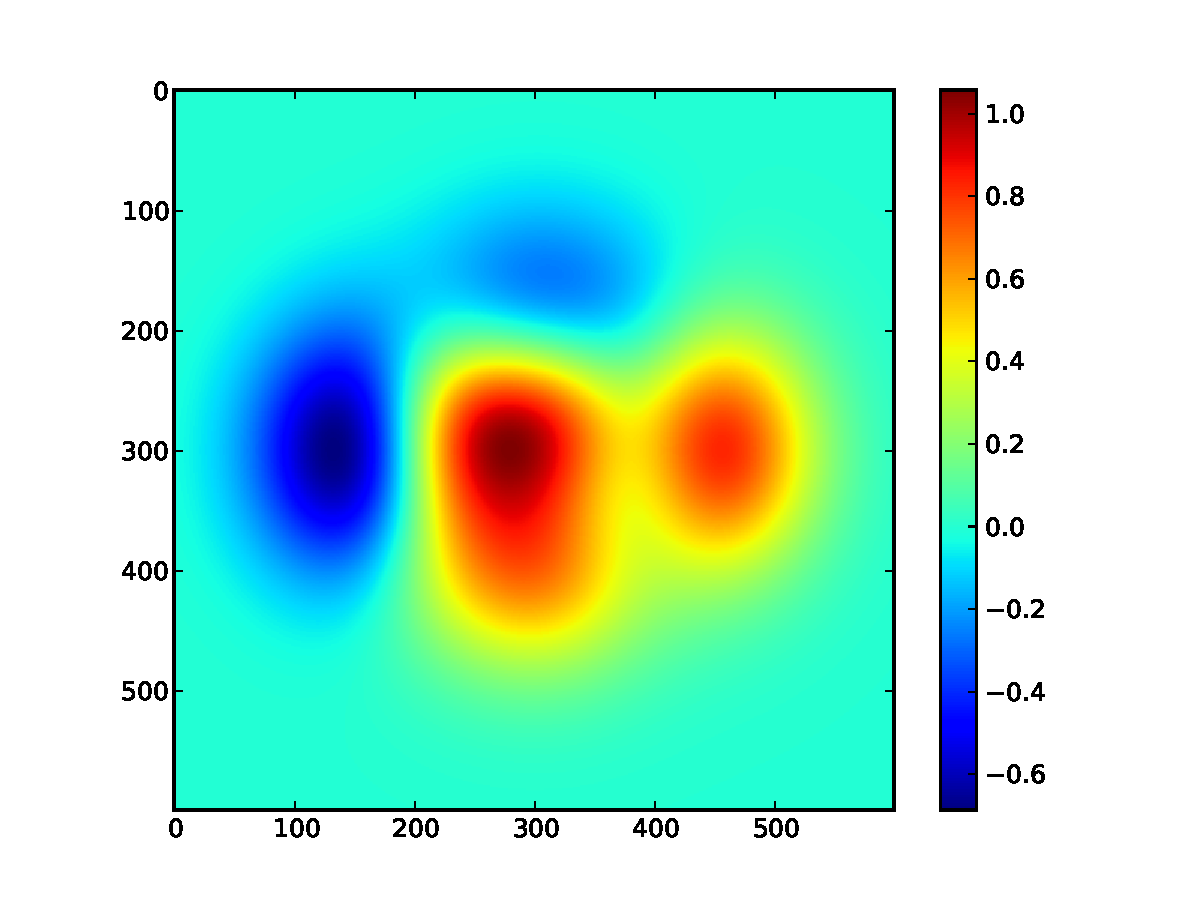
\includegraphics[width=0.6\textwidth]{Chapter-2/figs/color}
  \caption{A figure at the bottom of the page.}
  \label{fig:ch3.3}
\end{figure}
%
\lipsum[14-20]




%%---------------------------------------------------------------------------%%
%%  Bibliography 

%%  You can use the bibitem list.
%\bibliographystyle{unsrt}
%\begin{thebibliography}{99}
%\bibitem{cb02}
%Casella, G. and Berger, R.L. (2002)
%\newblock {\it Statistical Inference, Second Edition.}
%Duxbury Press, Belmont, CA.
%
%\bibitem{t06}
%Tsiatis, A.A. (2006)
%\newblock {\it Semiparametric Theory and Missing Data.}
%Springer, New York.
%
%\end{thebibliography}

%% or use BibTeX
\bibliography{YourName-thesis}{}
\bibliographystyle{plain}

%%---------------------------------------------------------------------------%%
% Appendices
\appendix

\chapter{Lorem Ipsum}

\section{A First Section}

\paragraph{Filler Text} \lipsum[1-6]
%
\begin{figure}
  \centering
  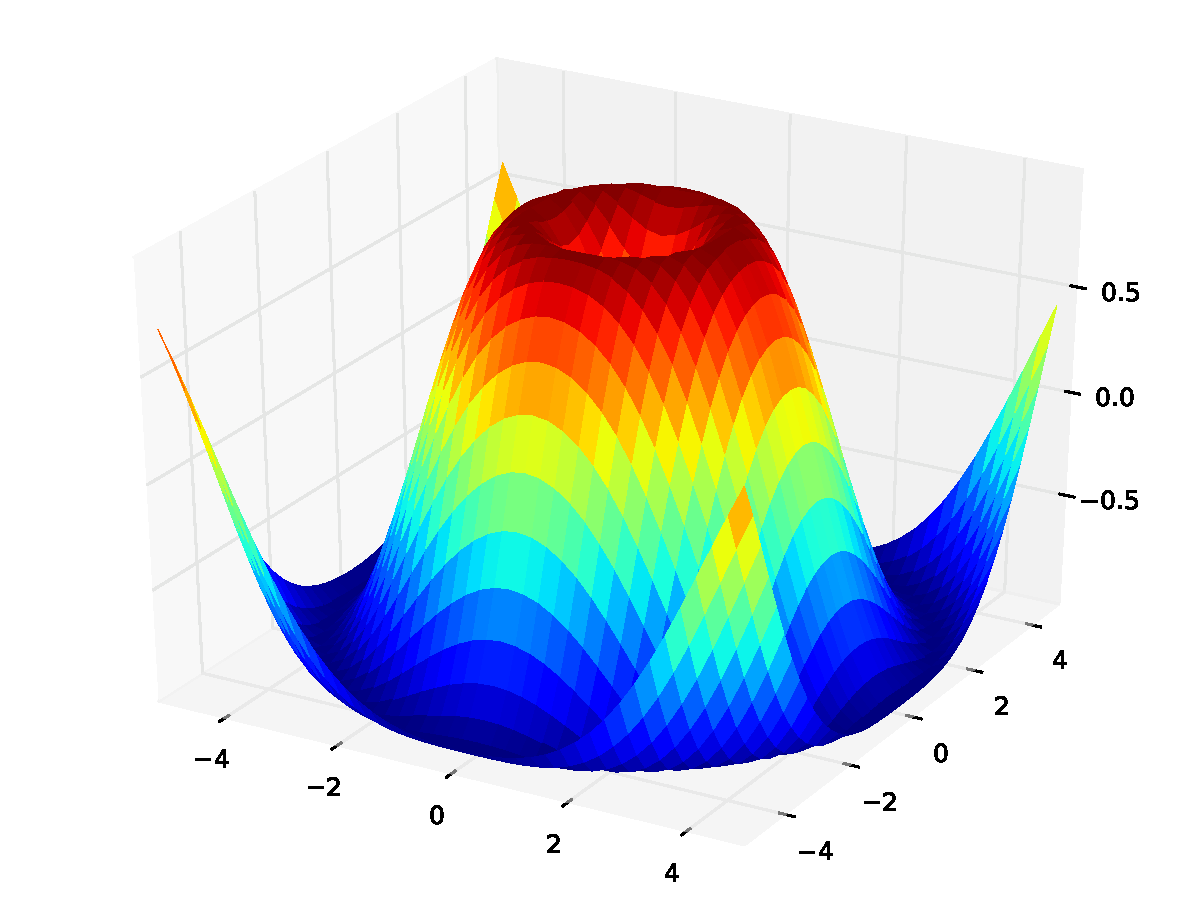
\includegraphics[width=0.6\textwidth]{Chapter-2/figs/threed}
  \caption{A figure in the appendix.}
  \label{fig:app}
\end{figure}
%
\lipsum[7-10]
\begin{table}
  \caption{A table in the appendix.}
  \label{tab:app}
  \begin{center}
    \begin{tabular}{lc}
      \toprule
      System & Author \\
      \midrule
      \TeX   & Donald Knuth   \\
      \LaTeX & Leslie Lamport \\
      \bottomrule
    \end{tabular}
  \end{center}
\end{table}
%

\section{A Second Section}

\lipsum[14-15]




%%---------------------------------------------------------------------------%%
\backmatter


\end{document}
